% One fixed nave-facing sanctuary for all three teaching forms. Coordinates
% locate feet on the shared drawing's treads; they are not dimensions.
\pgfdeclarelayer{asg labels}
\pgfsetlayers{main,asg labels}
\newlength{\ASGSceneWidth}
\newlength{\ASGSceneUnit}
\tikzset{
  asg label/.style={draw=black,fill=white,rounded corners=1pt,
    line width=.45pt,inner sep=2pt,align=center,
    font=\fontsize{7.2}{8.5}\selectfont\bfseries},
  asg route/.style={draw=black,line width=.8pt,dashed,
    -{Stealth[length=2mm,width=1.6mm]}},
  asg stop/.style={circle,draw=black,fill=white,line width=.6pt,
    minimum size=3.5mm,inner sep=1pt,
    font=\fontsize{7}{8}\selectfont\bfseries}}

\newcommand{\ASGBeginScene}[1]{%
  \setlength{\ASGSceneWidth}{#1}%
  \setlength{\ASGSceneUnit}{.01\ASGSceneWidth}%
  \begin{tikzpicture}[x=\ASGSceneUnit,y=\ASGSceneUnit]
    \path[use as bounding box] (0,1) rectangle (100,68);
    \node[anchor=south west,inner sep=0pt] at (0,0) {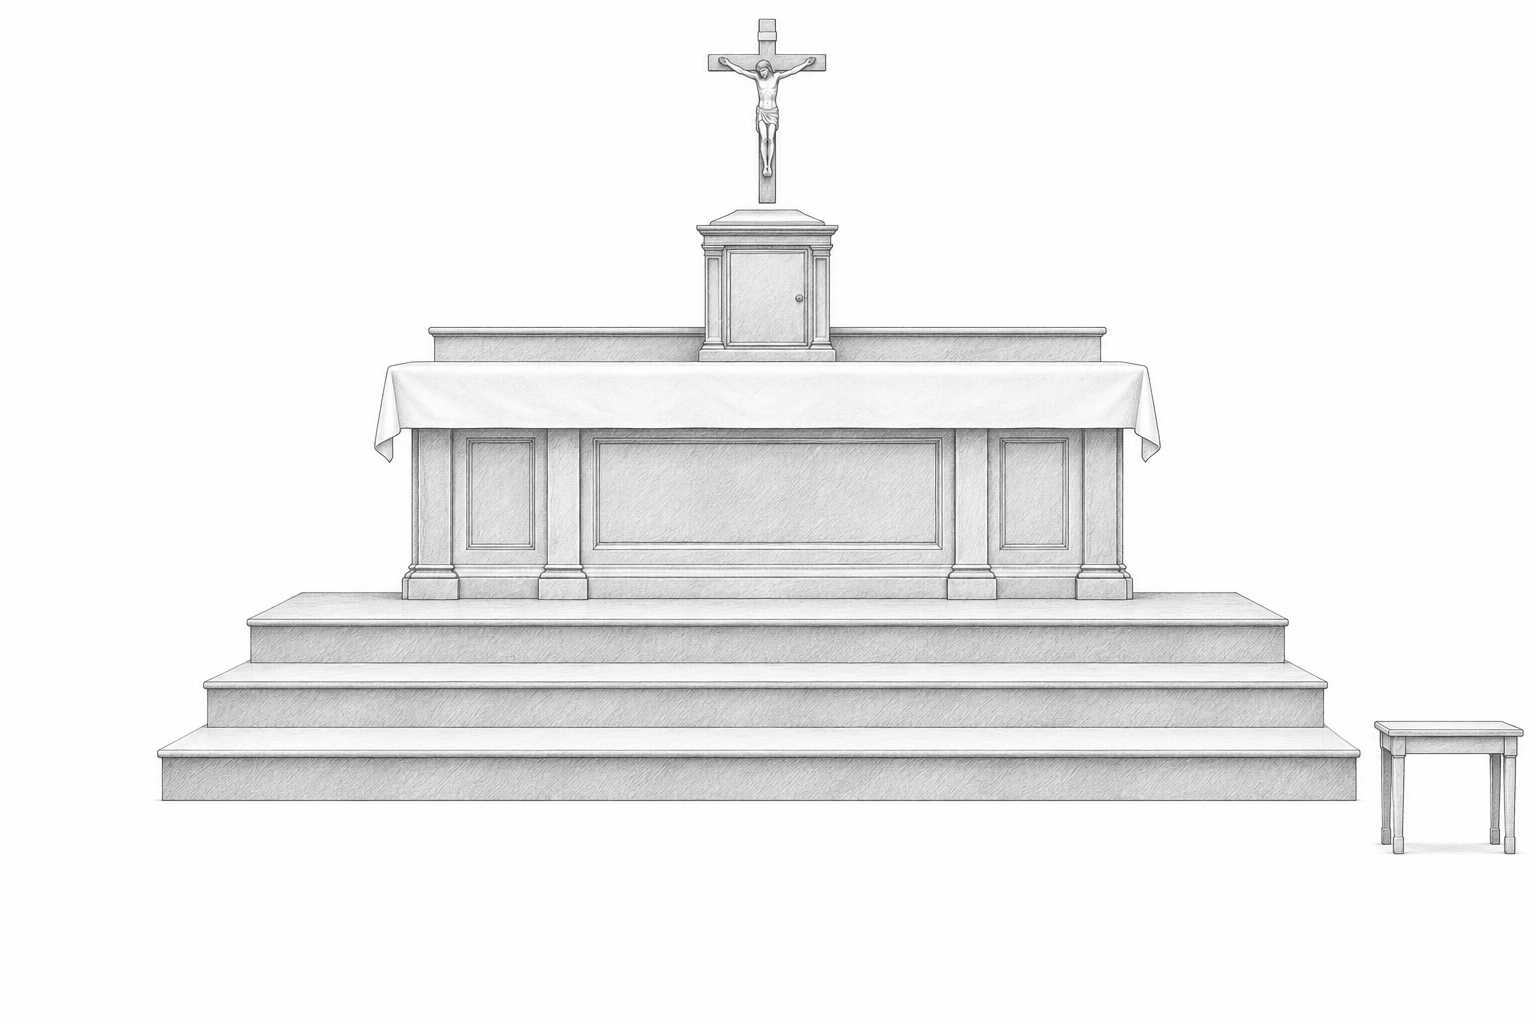
\includegraphics[width=\ASGSceneWidth]{liturgy/roman-rite/1962/reference/altar-server-guides/shared/artwork/pencil/ASG-ART-032-sanctuary-master.png}};
    \node[font=\fontsize{7}{8}\selectfont\bfseries,anchor=north west] at (2,66) {GOSPEL};
    \node[font=\fontsize{7}{8}\selectfont\bfseries,anchor=north east] at (98,66) {EPISTLE};
    \foreach \n/\y in {1/18.3,2/22.5,3/26.5}{%
      \node[asg stop] at (9,\y) {\n};}
    \node[font=\fontsize{6.6}{7.7}\selectfont,anchor=north] at (94,10.8) {CREDENCE};}
\newcommand{\ASGEndScene}{\end{tikzpicture}}

% Save the complete composed sanctuary once. A close view clips that box:
% architecture, appointments, actors and occlusion cannot drift independently.
\newsavebox{\ASGSceneSnapshot}
\newlength{\ASGZoomUnit}
\newcommand{\ASGSaveScene}[2]{%
  \sbox{\ASGSceneSnapshot}{\ASGBeginScene{#1}#2\ASGEndScene}}
\newcommand{\ASGShowSavedScene}{\usebox{\ASGSceneSnapshot}}
\newcommand{\ASGSceneViewport}[5]{%
  \begingroup
  \pgfmathsetlength{\ASGZoomUnit}{#5/(#3-#1)}%
  \begin{tikzpicture}[x=\ASGZoomUnit,y=\ASGZoomUnit]
    \begin{scope}
      \clip (0,0) rectangle (#3-#1,#4-#2);
      \node[anchor=south west,inner sep=0pt] at (-#1,-#2)
        {\resizebox{100\ASGZoomUnit}{!}{\ASGShowSavedScene}};
    \end{scope}
    \pgfresetboundingbox
    \path[use as bounding box] (0,0) rectangle (#3-#1,#4-#2);
    \draw[black!50,line width=.4pt] (0,0) rectangle (#3-#1,#4-#2);
  \end{tikzpicture}%
  \endgroup}

\newcommand{\ASGStandingServer}[3]{%
  \node[anchor=south,inner sep=0pt] at (#1,#2) {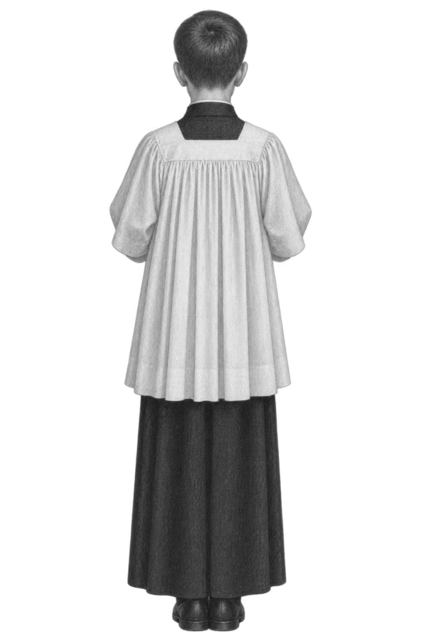
\includegraphics[height=23\ASGSceneUnit]{liturgy/roman-rite/1962/reference/altar-server-guides/shared/artwork/pencil/ASG-ART-033-server-standing.png}};
  \begin{pgfonlayer}{asg labels}\node[asg label,anchor=north] at (#1,#2) {#3};\end{pgfonlayer}}
\newcommand{\ASGKneelingServer}[3]{%
  \node[anchor=south,inner sep=0pt] at (#1,#2) {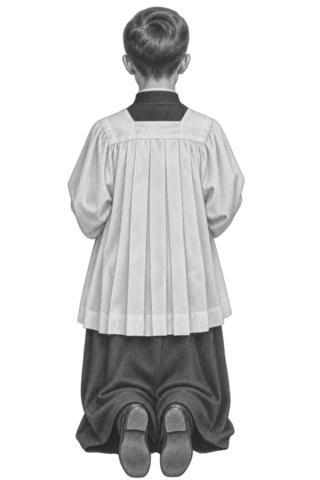
\includegraphics[height=16\ASGSceneUnit]{liturgy/roman-rite/1962/reference/altar-server-guides/shared/artwork/pencil/ASG-ART-034-server-kneeling.png}};
  \begin{pgfonlayer}{asg labels}\node[asg label,anchor=north] at (#1,#2) {#3};\end{pgfonlayer}}
\newcommand{\ASGPriest}[3]{%
  \node[anchor=south,inner sep=0pt] at (#1,#2) {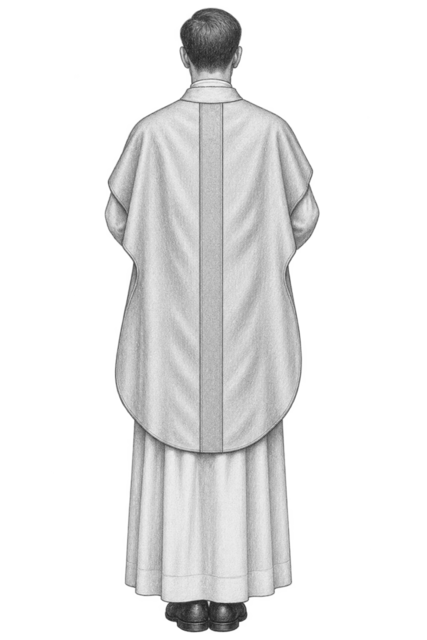
\includegraphics[height=28\ASGSceneUnit]{liturgy/roman-rite/1962/reference/altar-server-guides/shared/artwork/pencil/ASG-ART-035-priest-standing.png}};
  \begin{pgfonlayer}{asg labels}\node[asg label,anchor=north] at (#1,#2) {#3};\end{pgfonlayer}}
\newcommand{\ASGServerFacingLeft}[4][0]{%
  \node[anchor=south,inner sep=0pt] at (#2,#3) {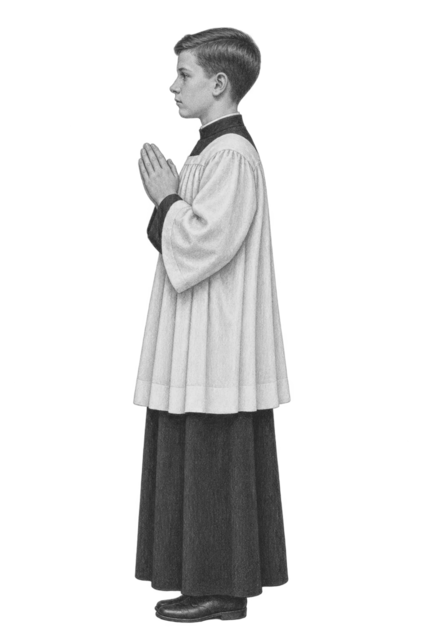
\includegraphics[height=23\ASGSceneUnit]{liturgy/roman-rite/1962/reference/altar-server-guides/shared/artwork/pencil/ASG-ART-037-server-facing-left.png}};
  \begin{pgfonlayer}{asg labels}\node[asg label,anchor=north] at (#2,#3-#1) {#4};\end{pgfonlayer}}
\newcommand{\ASGPriestFacingRight}[3]{%
  \node[anchor=south,inner sep=0pt] at (#1,#2) {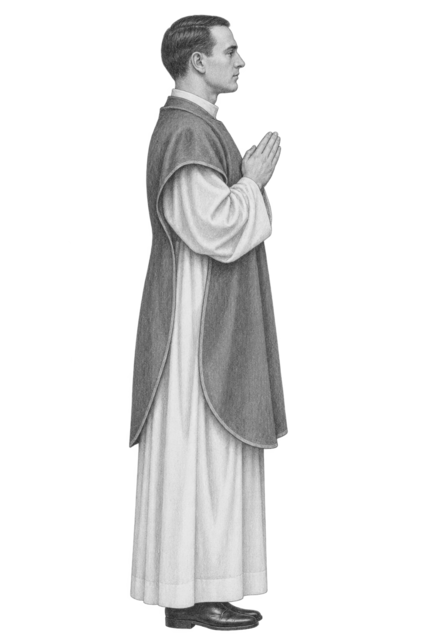
\includegraphics[height=28\ASGSceneUnit]{liturgy/roman-rite/1962/reference/altar-server-guides/shared/artwork/pencil/ASG-ART-038-priest-facing-right.png}};
  \begin{pgfonlayer}{asg labels}\node[asg label,anchor=north] at (#1,#2) {#3};\end{pgfonlayer}}
\newcommand{\ASGCandle}[1]{%
  \node[anchor=south,inner sep=0pt] at (#1,45) {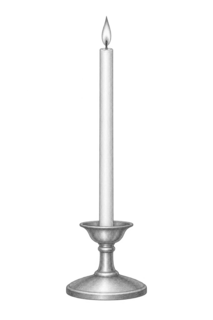
\includegraphics[height=11\ASGSceneUnit]{liturgy/roman-rite/1962/reference/altar-server-guides/shared/artwork/pencil/ASG-ART-036-altar-candle.png}};}
\newcommand{\ASGLowCandles}{\ASGCandle{31}\ASGCandle{69}}
\newcommand{\ASGSungCandles}{%
  \ASGCandle{30}\ASGCandle{36}\ASGCandle{42}%
  \ASGCandle{58}\ASGCandle{64}\ASGCandle{70}}
\newcommand{\ASGStation}[3]{\begin{pgfonlayer}{asg labels}\node[asg label] at (#1,#2) {#3};\end{pgfonlayer}}
\newcommand{\ASGMissalGospel}{\draw[thin] (37,43) -- (37,59);\ASGStation{37}{60}{MISSAL}}
\newcommand{\ASGPairPlan}[2]{%
  \begin{pgfonlayer}{asg labels}
  \filldraw[fill=white,draw=black!60] (12,24) rectangle (43,47);
  \node[font=\fontsize{6.5}{7.5}\selectfont\bfseries] at (27.5,44) {ABOVE: SIDE BY SIDE};
  \node[asg label] at (18,33) {P};
  \node[asg label] at (34,38) {#1};
  \node[asg label] at (34,28) {#2};
  \draw[-{Stealth[length=1.2mm]}] (28,38) -- (22,35);
  \draw[-{Stealth[length=1.2mm]}] (28,28) -- (22,31);
  \end{pgfonlayer}}
\newcommand{\ASGStop}[3]{\node[asg stop] at (#1,#2) {#3};}

\newcommand{\ASGOrientationKey}{%
  \par\smallskip\noindent\textbf{Look from the nave toward the altar.}
  Gospel stays picture-left; Epistle stays picture-right. The same altar,
  three levels and credence remain in every position view: 1 is the lowest
  step, 2 the second step, and 3 the predella. Lettered circles on a dashed
  route are successive stops, not extra people. Figures show the named
  standing or kneeling station; close views teach the hand action.
  The actual distances, reverences and side lanes are rehearsed locally.
  \par\smallskip}

\newcommand{\ASGMovementFields}[5]{%
  \par\smallskip\noindent{\small
  \textbf{Cue:} #1\quad\textbf{Who / object:} #2\par
  \textbf{Route:} #3\par
  \textbf{Finish:} #4\par
  \textbf{Waiting:} #5\par}\smallskip}
